\section{Home-Page - Rollen:Alle}
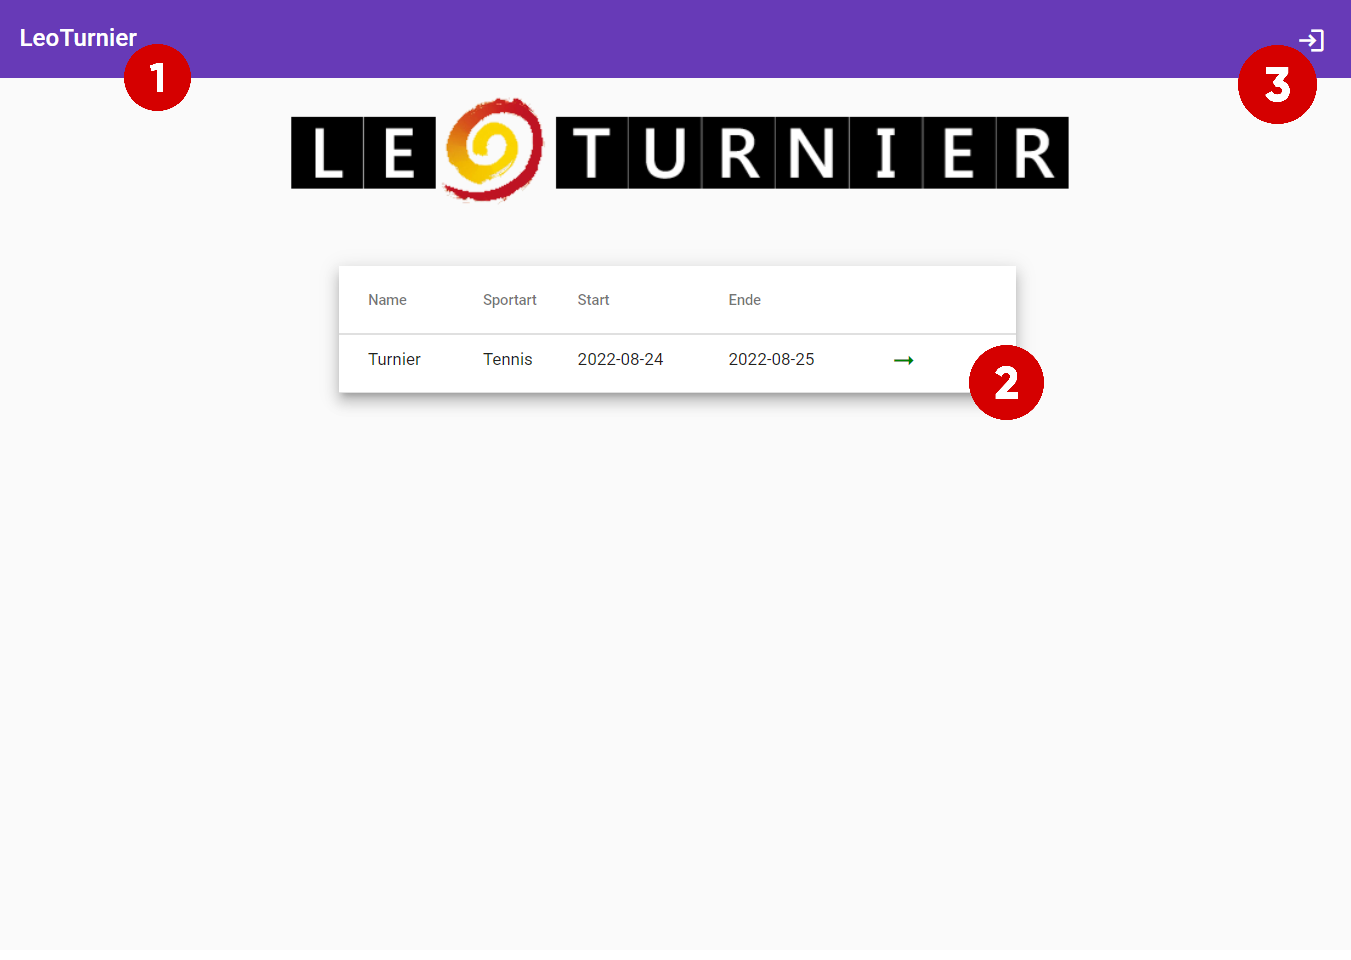
\includegraphics[scale=0.4]{pics/user-guide/homepage.png}
\bigskip


\includegraphics[scale=0.05]{pics/user-guide/numbers/number-1.png} \begin{LARGE} Titel \end{LARGE}

Links oben wird dauerhaft der Titel LeoTurnier gezeigt dieser dient auch gleichzeitig als Homebutton,
also kommt man per Knopfdruck immer wieder auf diese Seite.
\bigskip


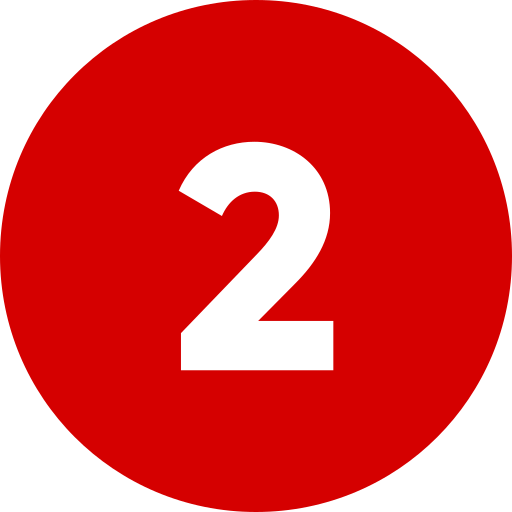
\includegraphics[scale=0.05]{pics/user-guide/numbers/number-2.png} \begin{LARGE} Laufenden Turniere \end{LARGE}

In dieser Tabelle werden alle laufenden Turniere angezeigt. Zu jedem Turnier werden die Sportart, das Startdatum und das Enddatum angezeigt,
sollten diese eingetragen sein. (\textit{Nur der Name und der Modus sind zur Erstellung nötig})
\bigskip

\newpage
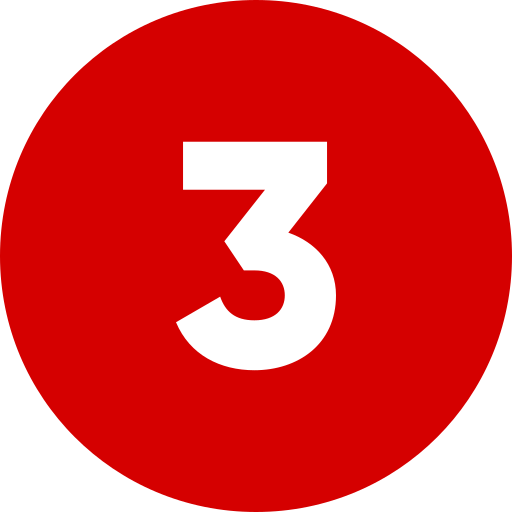
\includegraphics[scale=0.05]{pics/user-guide/numbers/number-3.png} \begin{LARGE} Login Button \end{LARGE}

Um Turniere zu erstellen und verwalten zu können ist es nötig sich vorher einzuloggen. Mit diesem Button sollten Sie direkt zum Keycloak weitergeleitet werden um sich mit ihrem Username und Password zu authorisieren.
Danach werden Sie zur Login-Page(5.3) weitergeleitet werden.
\section{Tournament-View-Page}
\section{Login-Page}
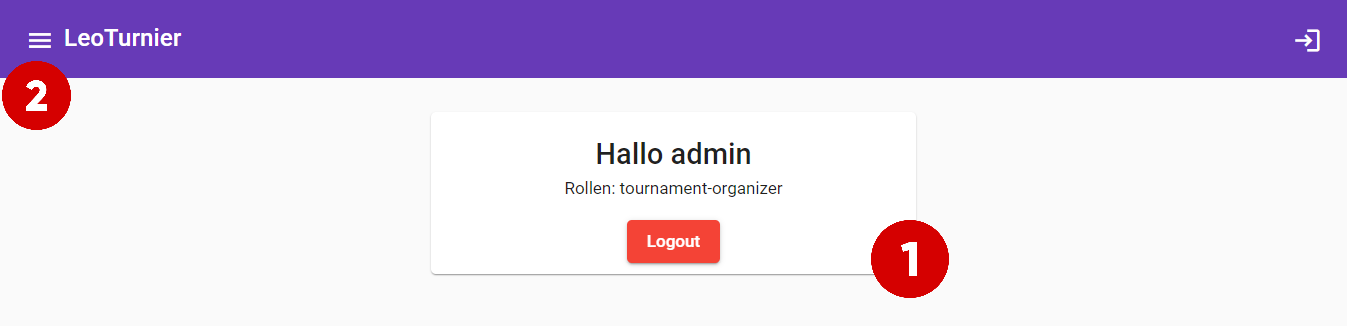
\includegraphics[scale=0.4]{pics/user-guide/login-page.PNG}
\bigskip


\includegraphics[scale=0.05]{pics/user-guide/numbers/number-1.png} \begin{LARGE} Rollen und Logout Button \end{LARGE}

Hier finden Sie alle Ihnen zugewiesenen Rollen sowie einen Logout-Button der ihre Session beendet und Sie zurück zur Home-Page leitet.
\bigskip

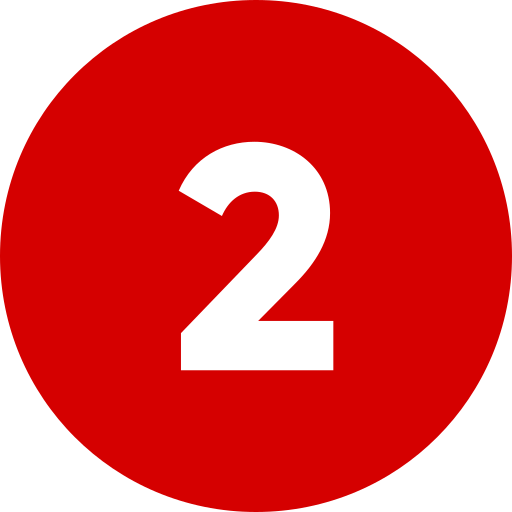
\includegraphics[scale=0.05]{pics/user-guide/numbers/number-2.png} \begin{LARGE} Navigation-Burger \end{LARGE}

Nachdem Sie jetzt eingeloggt sind erscheint oben rechts ein Nav-Burger. Per Knopfdruck zeigt dieser Ihnen nun eine Liste aller Pages die zur
Turnierverwaltung nötig sind.
\section{Player-Page}
\section{Team-Page}
\section{Tournament-Page}
\section{Match-Overview-Page} 